
\section{Developing mirror neurons}

\ifverbose
The latest instantiation of the ``general principle'' we would like to
dwell upon is related to mirror neurons. It turns out that the causal
chain here is more compliceted. This requires a more complicated
structure to support it.
\fi

%(some are mentioned in the conclusions)
Poking moves us one step outwards on a causal chain away from the
robot and into the world, and gives a simple experimental procedure
for segmenting objects.  There are many possible elaborations of this
method, all of which lead to a
vision system that is tuned to acquiring data about an object by
seeing it manipulated by the robot.  An interesting question then is
whether the system could extract useful information from seeing an
object manipulated by someone else.  In the case of poking, the robot
needs to be able to estimate the moment of contact and to track the arm
sufficiently well to distinguish it from the object being poked.  We
are interested in how the robot might learn to do this.  One approach
is to chain outwards from an object the robot has poked.  If someone
else moves the object, we can reverse the logic used in poking --
where the motion of the manipulator identified the object -- and
identify a foreign manipulator through its effect on the object.

%%%CHANGE%%%
We designed two experiments that use poking and the visual
segmentation described in the previous sections to probe 
the structure of objects and control \ahhbehavior{} on the basis of
their affordances. Further, although poking gives us a simple 
procedure for segmenting objects, the procedure would be 
nevertheless inconvenient in many situations if we had to poke an 
object every time we needed to grasp it. A better solution is that 
of learning from experience about the \ahhbehavior{}, visual appearance and 
physical properties of objects.

In the first experiment the robot poked a small set of objects 
(an orange juice bottle, a toy car, a cube, and a \ahhcolor{}ed ball) using 
one of four possible actions (the motor repertoire). Actions are 
indicated for convenience as pull in, side tap, push away, and back 
slap (see for example figure \ref{fig:poking-segmentation}). 
The toy car and the bottle have a definite principal axis that 
can be easily extracted from the segmented image. They also tend to 
roll along a definite direction with respect to their principal axis. 
These visual and physical properties of the objects can be acquired 
automatically by the robot simply by poking the same object many times 
(about 100 in our experiment). The results are shown in figure 
\ref{fig:affordances}. We plotted there the estimated probability 
of observing each of the objects rolling along a particular direction 
with respect to its principal axis. Different trials were clustered 
using \ahhcolor{} information. In fact, in this case, \ahhcolor{} allows 
distinguishing one object from another. The next step is that of 
acquiring an understanding of poking. This is easily obtained from 
the same training set. Instead of considering each object separately 
here, we simply measured the average direction of movement given a 
certain action. In \ahhpractice{}, the robot automatically learns that 
poking from the left causes the object to slide/roll to the right. 
A similar consideration applies to the other actions.

%
%
\begin{figure}[tb]
\begin{center}
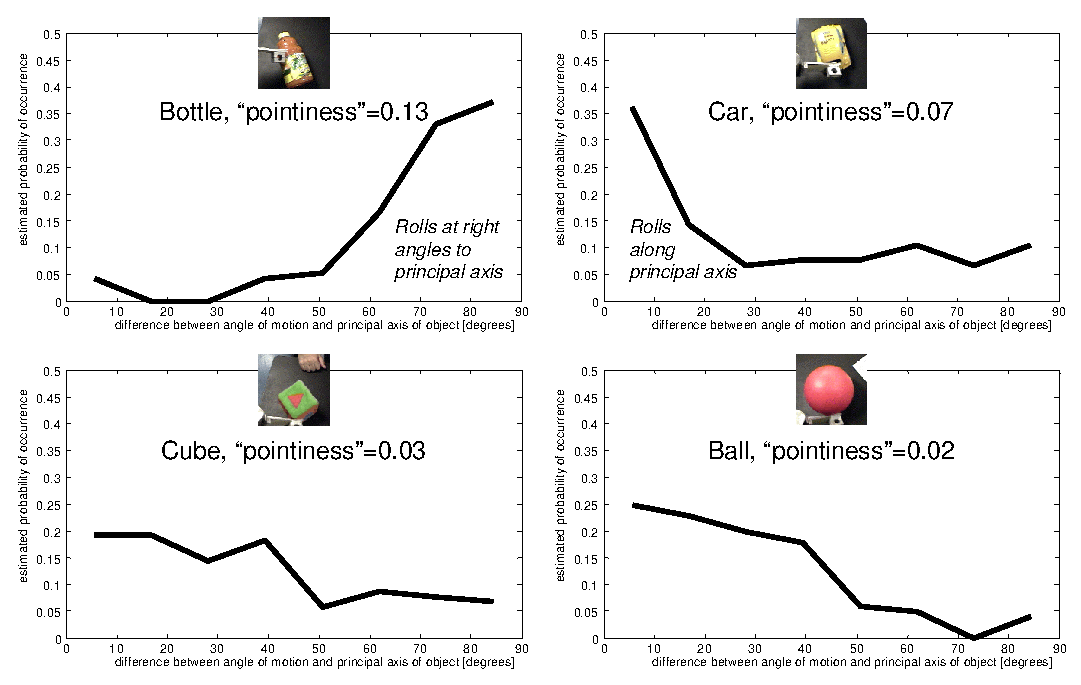
\includegraphics[width=\columnwidth]{affordances.eps}
\caption{ 
\label{fig:affordances}
%
%
Probability of observing a roll along a particular direction for the set of
four objects used in Cog's experiments. Abscissae represent the difference
between the principal axis of the object and the observed direction of movement.
Ordinates are the estimated probability.
}
\end{center}
\end{figure}
%
%

After the training stage, if one of the known objects is presented to Cog, the 
object is recogn\ize{}d, local\ize{}d and its orientation estimated (principal 
axis). Recognition and local\iz{}ation are based on the same \ahhcolor{} 
segmentation algorithm used during learning. Cog then uses its 
understanding of the affordance of the object (figure \ref{fig:affordances}) 
and of the geometry of poking to make the object roll. The whole local\iz{}ation 
procedure has an error between $10^{\circ}$ and $25^{\circ}$ which proved 
to be enough for our experiment. We performed a simple qualitative test of 
the overall performance of the robot. Out of 100 trials the robot made 15 
mistakes. Twelve of them were due to imprecise control: e.g. the end point 
touched the object earlier than expected moving the car outside the field of 
view. The remainders (3) were genuine mistakes due to misinterpretation of 
the object position/orientation.

This experiment represents an analogue of the response of F5/AIP as 
explained in Arbib's model \cite{fagg-arbib-1998} in that a specific 
structure of the robot detects the affordance of the object and links 
it to the generation of \ahhbehavior{}. This is also the first stage of 
the development of more complex \ahhbehavior{}s which relies on the understanding 
of objects as physical entities with specific properties.

With the knowledge about objects collected in the previous experiment
we can then set up a second experiment. In fact, the same visual processing 
used for analyzing an active poking has been used to detect a contact and 
segment the object from the manipulator. 
The first obvious thing the robot can do then is to identify the action 
just observed with respect to its motor vocabulary. It is easily done by 
comparing the displacement of the object with the four possible actions and 
by choosing the action whose effects are closer to the observed displacement. 
This procedure is orders of magnitude simpler than trying to completely 
\ahhcharacterize{} the action in terms of the observed kinematics of the movement. 
Here the complexity of the data we need to obtain is somewhat proportional 
to the complexity of the goal rather than that of the structure/skill of 
the foreign manipulator.

The robot can also mimic the observed \ahhbehavior{} if it happens to see the 
same object again. This requires another bit of information. The angle 
between the affordance of the object (\ahhpreferred{} direction of motion) and the 
observed displacement is measured. During mimicry the object is local\ize{}d as 
in the previous experiment and the action which is more likely to 
produce the same observed angle (relative to the object) is generated. 
If, for example, the car was poked at right angle with respect to its principal 
axis Cog would mimic the action by poking the car at right angle. In spite 
of the fact that the car \ahhpreferred{} \ahhbehavior{} is to move along its principal 
axis. Examples of observation of poking and generation of mimicry actions are 
shown in figure \ref{fig:observed-action} and \ref{fig:mimicked-action}.

%
%
\begin{figure}[tb]
\begin{center}
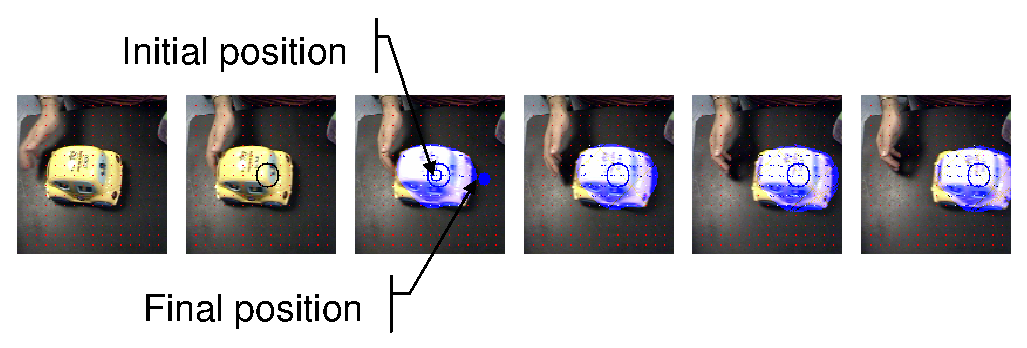
\includegraphics[width=\columnwidth]{observed-action.eps}
\caption{ 
\label{fig:observed-action}
%
%
An example of observed sequence. Frames around the instant of impact are shown.
Initial and final position after 12 frames is indicated.
}
\end{center}
\end{figure}
%
%

%
%
\begin{figure}[tb]
\begin{center}
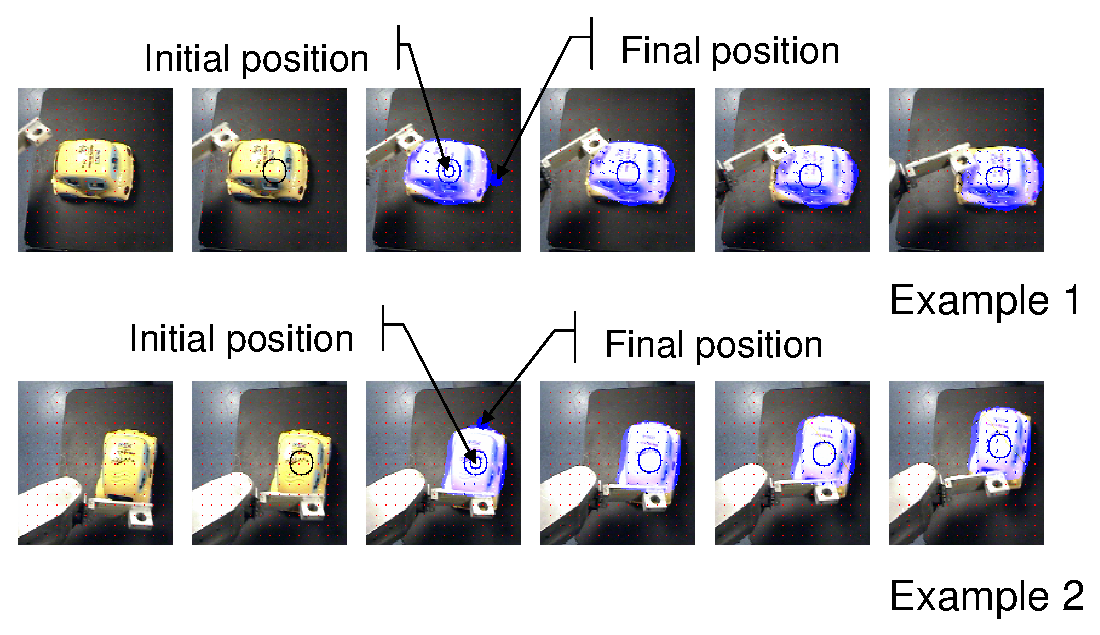
\includegraphics[width=\columnwidth]{mimicked-action.eps}
\caption{ 
\label{fig:mimicked-action}
%
%
Two examples of mimicry following the observation of figure \ref{fig:observed-action}. 
Cog mimics the goal of the action (poking along the principal axis) rather than
the trajectory followed by the toy car.
}
\end{center}
\end{figure}
%
%






\ifverbose
Poking is an ideal testbed for future work on this, since it is much
simpler than full-blown object manipulation and would only require a
very simple model of the foreign manipulator to work.
There is considerable precedent in the biological literature for a
strong connection between viewing object manipulation performed by
either oneself or another \cite{wohlsclager02human}. Also
the role of object in the understanding of action performed by others
has been investigated~\cite{woodward98infants}. In a series of
experiments Woodward and colleagues elucidated the contribution that
seeing an object makes for 5, 6, and 9 month old infants. They
provided evidence that the object and the goal-directness of the
action represent an important component in the understanding of the
intentions of others.
\fi

\ifverbose
At the neural level, we already mentioned the presence of neurons in
F5 that have a very specific response when an object is either fixated
or manipulated (canonical neurons). Grossly simplifying, we might
think of canonical neurons as an association table of
grasp/manipulation (action) types with object (vision) types.
\fi

As we described before, mirror neurons respond when either watching 
somebody else performing a manipulative action or when actually 
manipulating an object. They can be thought of as an 
association map which links together the observation of a manipulative 
action performed by somebody else with the neural representation of one's 
own action. The question of whether a mirror-like representation can be
autonomously developed by the robot (or a human for that matter) can
then be answered. The association map can be constructed by
identifying when the goal and the object are the same irrespective of
who is the actor. Actions that lead to the same consequences are thus
part of the same equivalence class.  This is exactly what mirror neurons
represent.

\begin{figure}[tb]
\begin{center}
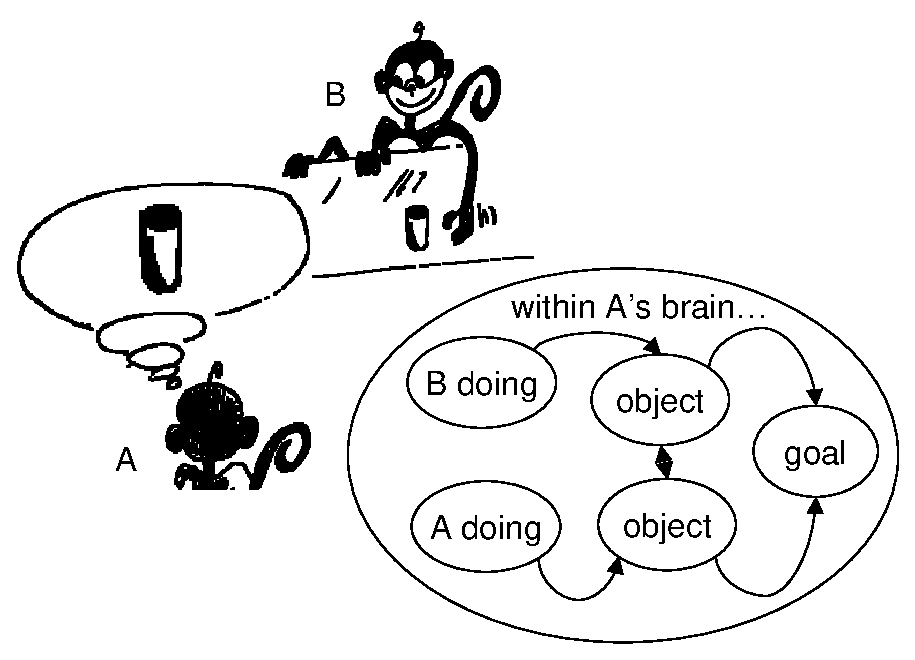
\includegraphics[width=10cm]{mirror-monkey.eps}
\caption{ 
\label{fig:mirror-monkey}
%
Mirror neurons and causality: from the observer's point
of view (A), understanding B's action means mapping it onto the
observer's own
motor repertoire. If the causal chain leading to the goal is already
in place (lower branch of the graph) then the acquisition of a
mirror neuron for this particular action/object is a matter of
building and linking the upper part of the chain to the lower one.
There are various opportunities to reinforce this link either at the object
level, at the goal level or both. 
%%Developmentally we can explain
%%mirror neurons only if we take into account another class of neurons
%%(called canonical) which in \ahhpractice{} describes the lower branch of the
%%graph.
%
}
\end{center}
\end{figure}


\ifverbose
There is considerable precedent in the literature for a strong
connection between viewing object manipulation performed by either
oneself or another \cite{wohlsclager02human}.  As we already mentioned
F5 contains a class of neurons called canonical neurons that have a
very specific response when an object is being either manipulated or
fixated.  Grossly simplifying, we might think of canonical neurons as
an association table of grasp/manipulation (action) types with object
(vision) types.  Another class of neurons called ``mirror neurons''
can then be thought of as a second-level association map which links
together the observation of a manipulative action performed by
somebody else with the neural representation of one's own action.
\fi

Figure~\ref{fig:mirror-monkey} shows this causal chain in action.
There are a series of interesting \ahhbehavior{}s that can be real\ize{}d based
on mirror neurons. Mimicry is an obvious application, since it
requires just this type of mapping between other and self in terms of
motor actions.  Another important application is the prediction of
future \ahhbehavior{} from current actions, or even inverting the causal
relation to find the action that most likely will get to the desired
consequence.

\ifverbose

for example, by observing the part of an action the robot or the
bioagent can come out with suitable expectations of the consequences
of that action. On the other hand, the inverse \ahhbehavior{} can also be
foreseen. The latter account to inverting the causal relation and
getting the action that most likely will get to the desired
consequence.

It might be argued that we need a two stages procedure to learn a
mirror representation, where we first learn ``something'' and only
subsequently we ``understand'' other people's \ahhbehavior{}. The actual
developmental course might not be such artificially staged. A slight
advantage must be given though to the initial step of self-learning,
the undestanding comes later.


This set of associations can be learnt autonomously (by a robot for
example) simply by a trial and error procedure and possibly with a
reinforcing signal to tell when a given grasp/manipulatory gesture was
successful if applied to a particular object.

We should not probably think of this association as describing in
detail the object being manipulated visually. Perhaps only features
relevant to manipulation are stored (e.g. size, orientation in space).
This representation is a ``pragmatic'' one describing only those
properties of objects are needed to apply a particular set of actions
to them. Affordances are a good psychological analogue of F5
canonical neurons.
\fi


\ifverbose
How does this relate to causation?  The two situations in some sense
share the same goal, and more practically share the same object.  The
whole procedure assumes a basic discrimination of size and shape of
objects (not necessarily categor\iz{}ation in traditional sense), and the
exploitation of the visual information to the understanding of the
grasp type. In some cases though the goal might be unambiguous, e.g. a
needle is very unlikely grasped with a full palm grasp, as well as a
box is not grasped with a pinch grip. These are the most informative
allowing for the best discrimination of action type from the visual
perspective.
\fi

\ifverbose
The definition of imitation we gave here implicitly focus on imitating
the goal rather than the precise trajectory. This automatically takes
into account any difference in body structure between the actor and
the observer.

Of course, manipulation as in poking can lead to a better
understanding of the physical properties of objects not directly
amenable to visual exploration such as mass, roughness, softness, etc.
\fi

\ifverbose
\begin{figure}[tbh]
\begin{center}
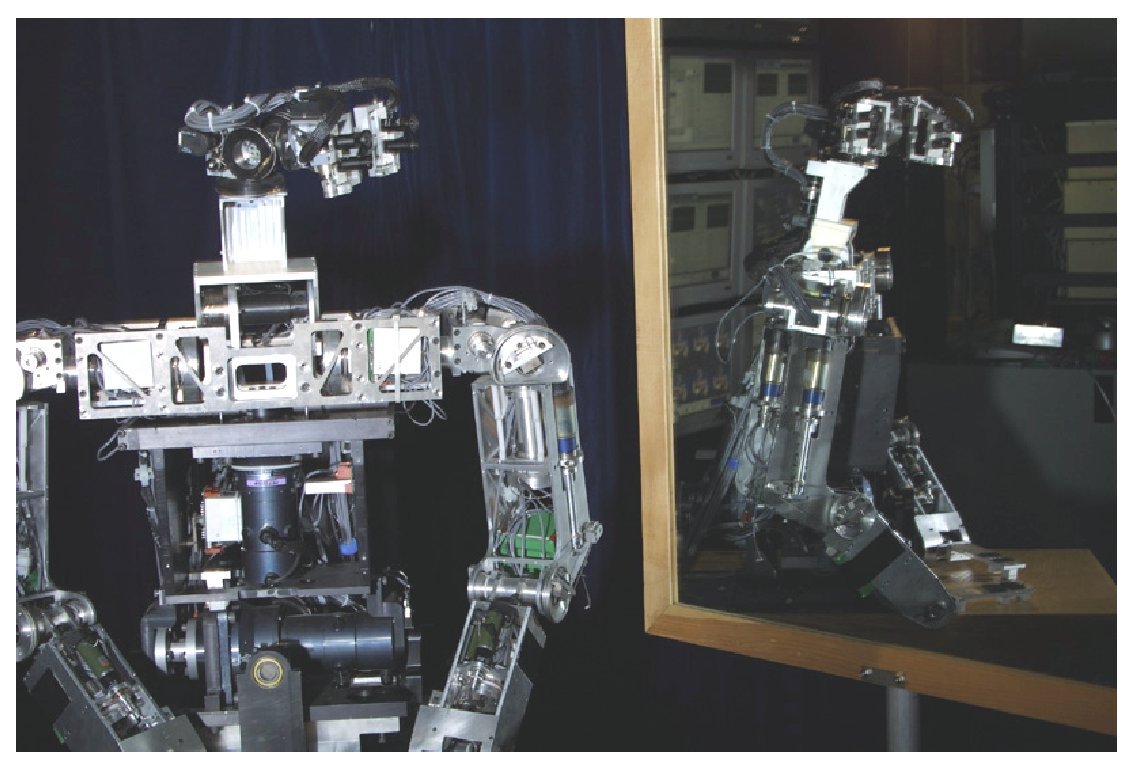
\includegraphics[width=\columnwidth]{mirror-cog.eps}
\caption{ 
\label{fig:mirror-cog}
%
The ultimate goal of this work is for our robot to follow chains of
causation outwards from its own simple body into the complex world.
%
}
\end{center}
\end{figure}
\fi
